% --------------------------------------------------------------------------- %
% Poster for the ECCS 2011 Conference about Elementary Dynamic Networks.      %
% --------------------------------------------------------------------------- %
% Created with Brian Amberg's LaTeX Poster Template. Please refer for the     %
% attached README.md file for the details how to compile with `pdflatex`.     %
% --------------------------------------------------------------------------- %
% $LastChangedDate:: 2011-09-11 10:57:12 +0200 (V, 11 szept. 2011)          $ %
% $LastChangedRevision:: 128                                                $ %
% $LastChangedBy:: rlegendi                                                 $ %
% $Id:: poster.tex 128 2011-09-11 08:57:12Z rlegendi                        $ %
% --------------------------------------------------------------------------- %
\documentclass[a0paper,portrait]{baposter}

\usepackage{relsize}		% For \smaller
\usepackage{url}			% For \url
\usepackage{epstopdf}	% Included EPS files automatically converted to PDF to include with pdflatex

\usepackage[sfdefault]{roboto}  %% Option 'sfdefault' only if the base font of the document is to be sans serif
\usepackage[T1]{fontenc}
\usepackage{fontawesome}
\usepackage{enumitem}
\usepackage{adjustbox}
\usepackage{svg}
\usepackage[font=small,labelfont=bf]{caption} % Required for specifying captions to tables and figures
\usepackage{changepage}
\usepackage[nomessages]{fp}% http://ctan.org/pkg/fp
\usepackage{calc}% http://ctan.org/pkg/calc
\usepackage{amsmath}
\usepackage[outline]{contour}
\usepackage{tcolorbox}
\usetikzlibrary{arrows.meta}

% To remove once you work on your own project
\newcommand{\dummycontentabstract}{
	\LipsumPar{75}
}

\newcommand{\dummycontentintroduction}{
	\LipsumPar{4}
	\begin{minipage}{.45\textwidth}
		\lipsum[66]	
	\end{minipage}
	\begin{minipage}{.54\textwidth}
        \begin{center}
            \includesvg[width=.8\textwidth]{./imgs/shower_example}
            \captionof{figure}{Electromagnetic shower}
        \end{center}
	\end{minipage}
}

\newcommand{\dummycontentsomething}{
	\begin{center}
		\begin{tikzpicture}
			\node (img) {
				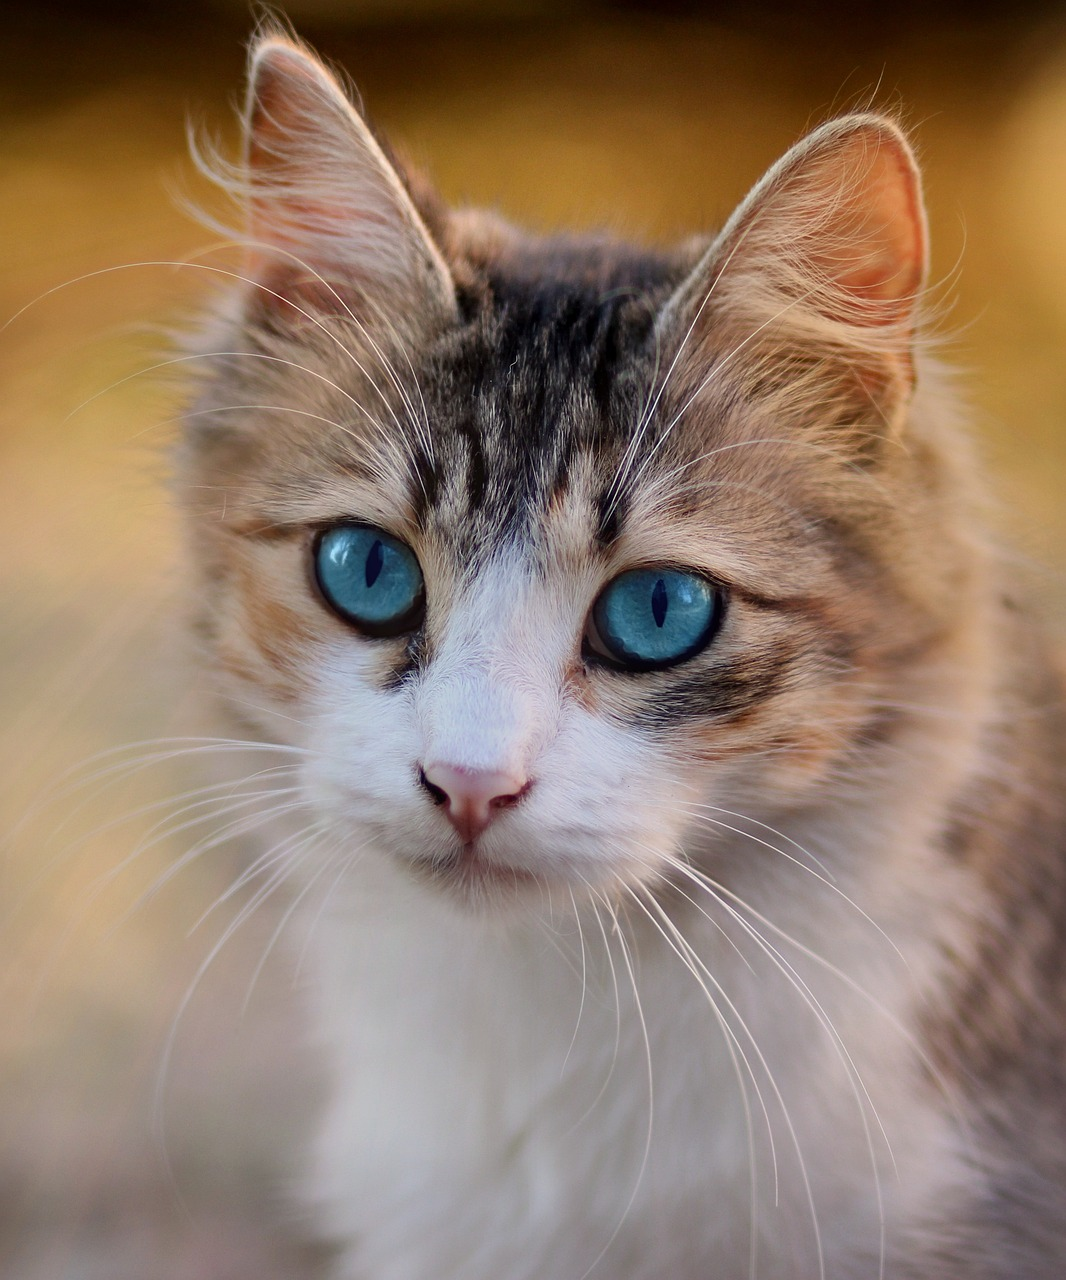
\includegraphics[width=.3\textwidth, trim={0, 5cm, 0, 2cm}, clip]{./imgs/cat.jpg}
			};
			\node (img) at (6,0) {
				\includesvg[width=.3\textwidth]{./imgs/bloch}
			};
		\draw[-{Triangle[width=30pt,length=20pt]}, line width=10pt, color=desyblue](2,0) -- (4, 0);	
		\end{tikzpicture}\\[.5cm]
		\begin{tikzpicture}
			\node (img) {
				\scalebox{1}[-1]{\includesvg[width=.3\textwidth]{./imgs/bloch}}
			};
			\node (img) at (6,0) {
				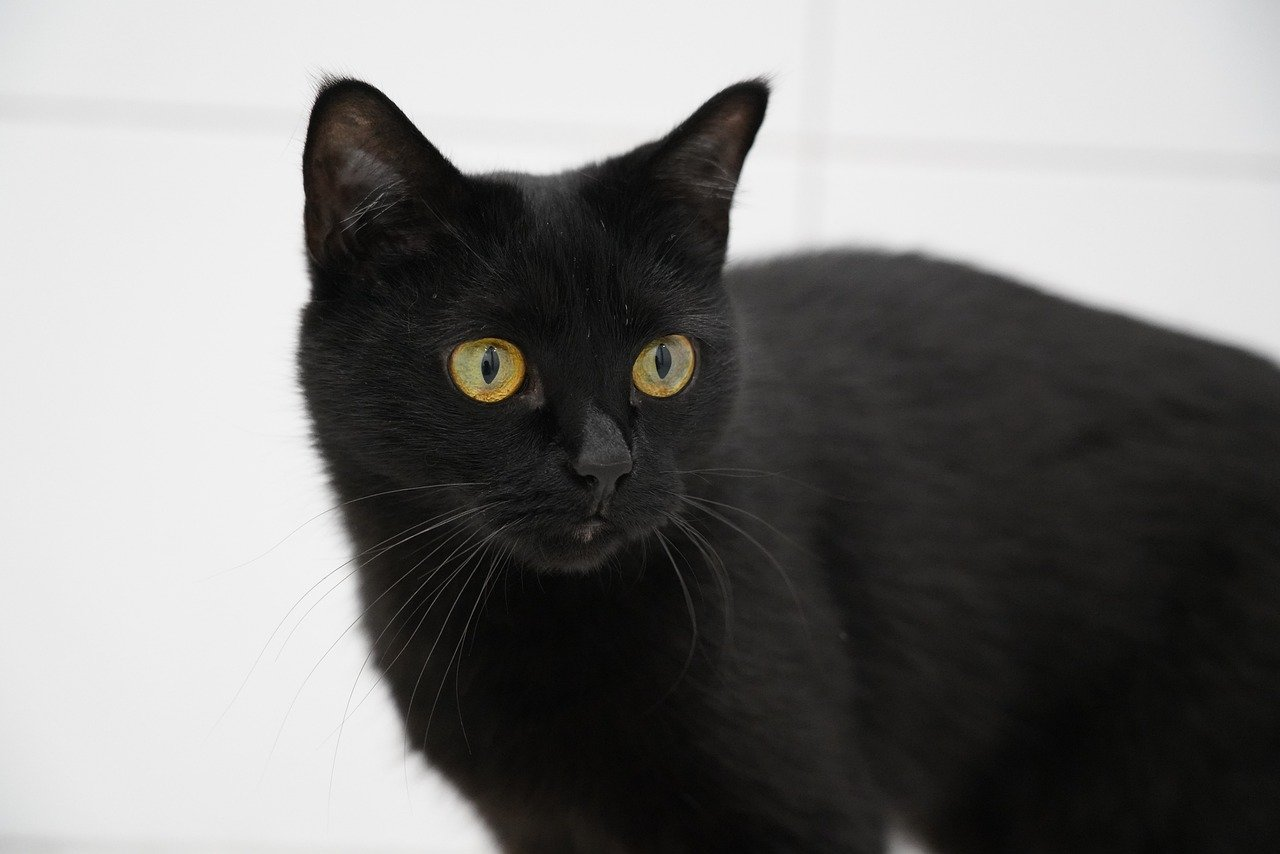
\includegraphics[width=.3\textwidth, trim={6cm, 0, 8cm, 0}, clip]{./imgs/cat_alt.jpg}
			};
		\draw[-{Triangle[width=30pt,length=20pt]}, line width=10pt, color=desyblue](2,0) -- (4, 0);	
		\end{tikzpicture}
		\captionof{figure}{A cat can be encoded into a \emph{Bloch sphere} and viceversa}
	\end{center}

	\LipsumPar{4}
}

\newcommand{\dummycontentsomethingelse}{
	\LipsumPar{4}
	\begin{center}
		\begin{tikzpicture}
			\node (img) {
				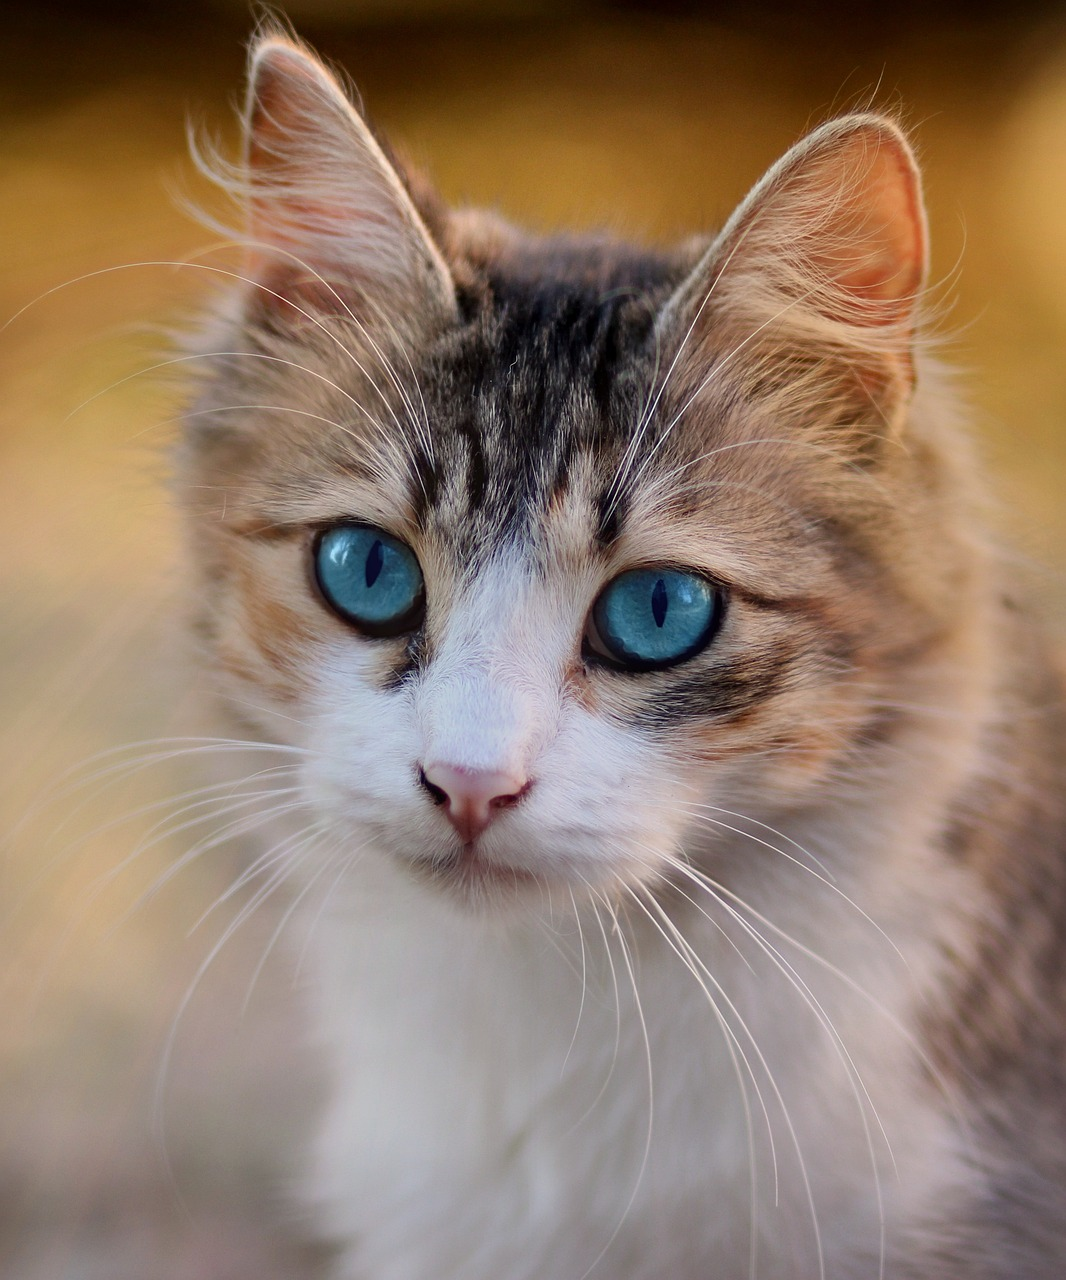
\includegraphics[width=.3\textwidth, trim={0, 5cm, 0, 2cm}, clip]{./imgs/cat.jpg}
			};
			\node (img) at (6,0) {
				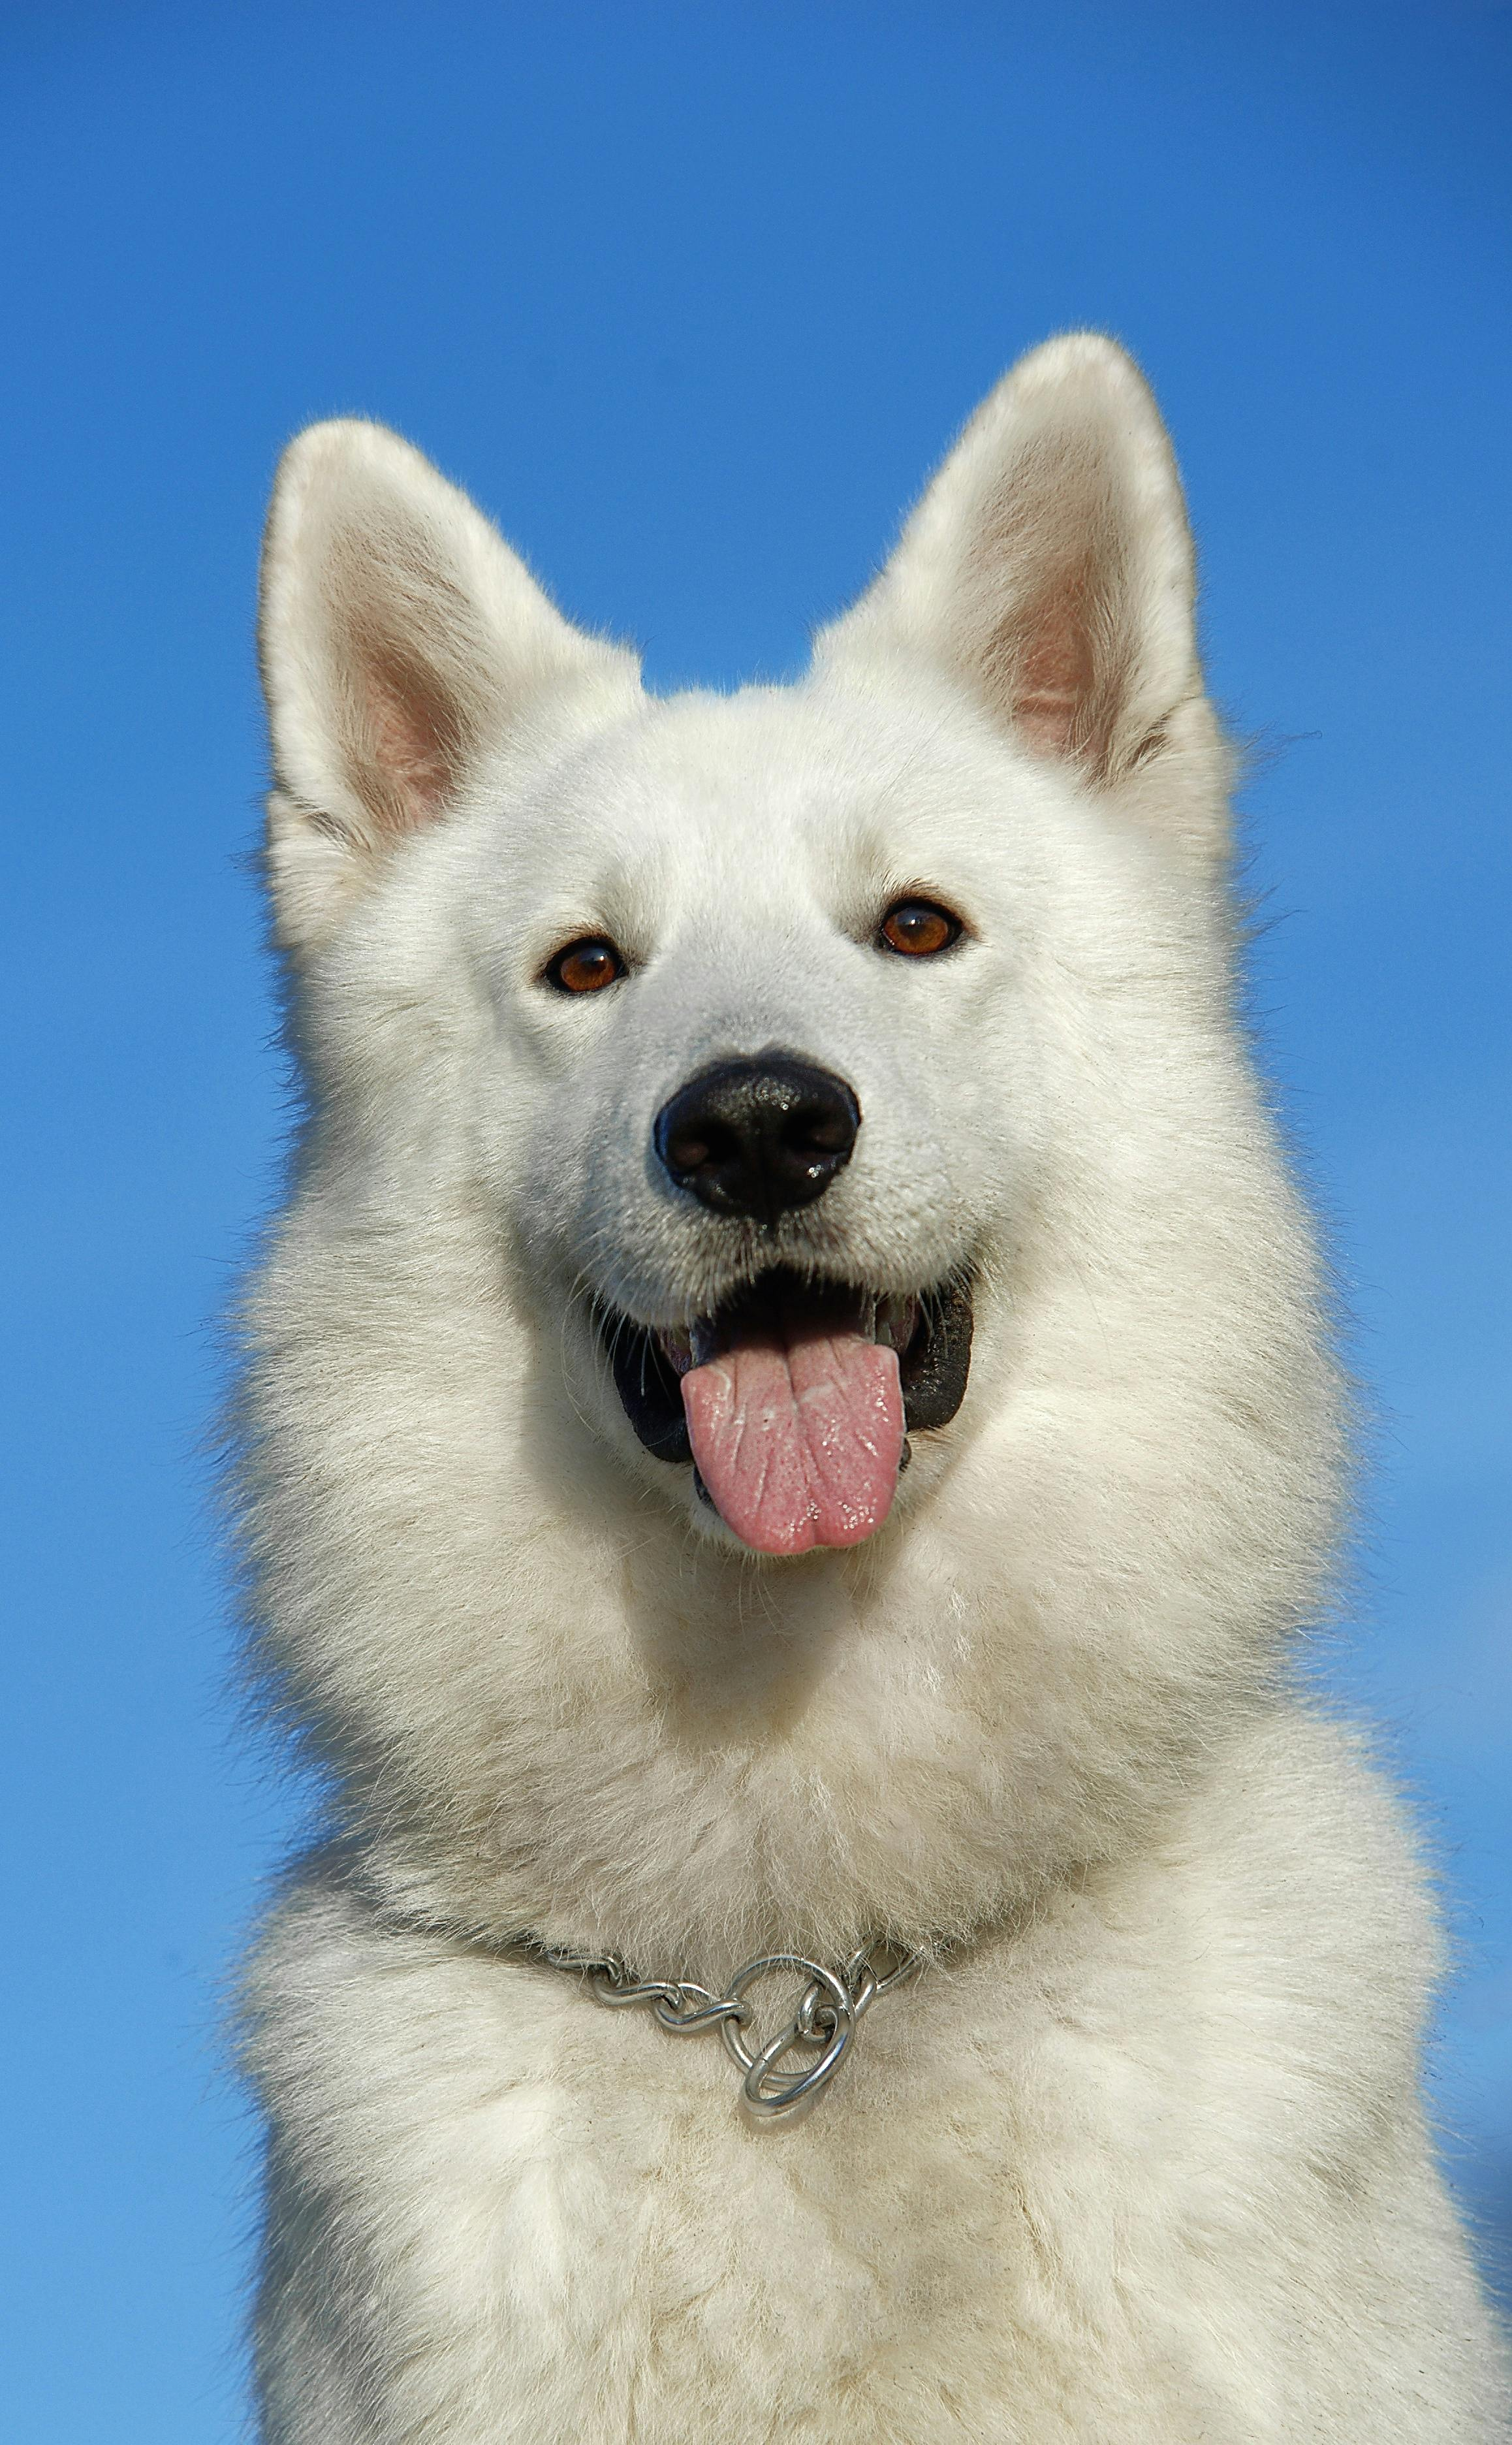
\includegraphics[width=.3\textwidth, trim={0, 27cm, 0, 18cm}, clip]{./imgs/dog.jpg}
			};
		\draw[-{Triangle[width=30pt,length=20pt]}, line width=10pt, color=desyblue](2,0) -- (4, 0);	
		\draw[line width=5pt, color=red](2,-.5) -- (4, .5);	
		\end{tikzpicture}
		\captionof{figure}{A cat is not a dog}
	\end{center}
	\LipsumPar{66}
	\begin{center}
		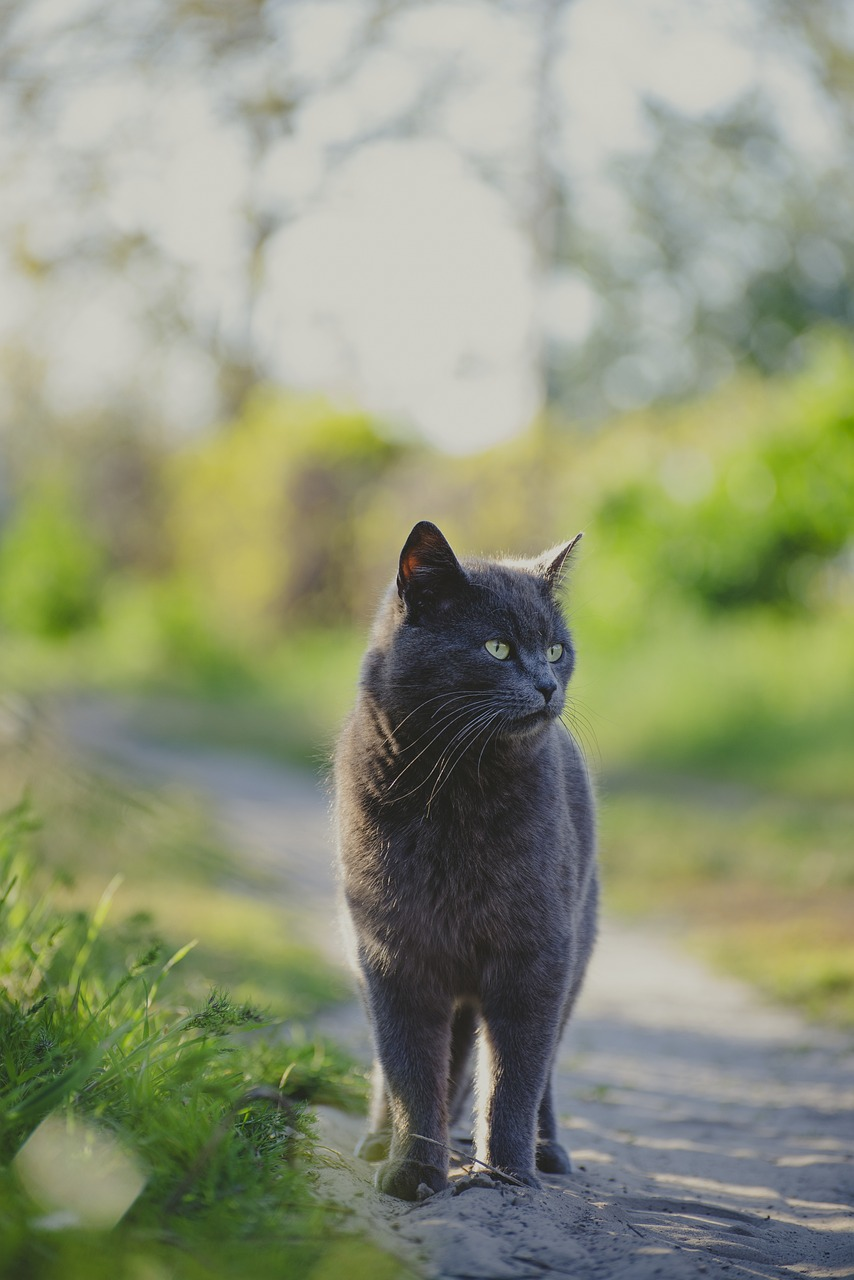
\includegraphics[width=.72\linewidth]{./imgs/cat_vertical.jpg}
		\captionof{figure}{A photo of a cute cat (I run out of ideas for things to add)}
	\end{center}
}
\usepackage{lipsum}

%%% Global Settings %%%%%%%%%%%%%%%%%%%%%%%%%%%%%%%%%%%%%%%%%%%%%%%%%%%%%%%%%%%

\graphicspath{{pix/}}	% Root directory of the pictures 
\tracingstats=2			% Enabled LaTeX logging with conditionals

%%% Color Definitions %%%%%%%%%%%%%%%%%%%%%%%%%%%%%%%%%%%%%%%%%%%%%%%%%%%%%%%%%

% Color codes taken from:
% https://quantum-zeuthen.desy.de/sites/sites_desygroups/sites_extern/site_quantum-zeuthen/content/e148955/e148956/DESYQuantum_Logoversions_eng.pdf
\definecolor{desyblue}{RGB}{0,159,223}
\definecolor{desyorange}{RGB}{243, 139, 60}

\definecolor{bordercol}{RGB}{40,40,40}
\definecolor{headercol1}{RGB}{186,215,230}
\definecolor{headercol2}{RGB}{80,80,80}
\definecolor{headerfontcol}{RGB}{0,0,0}
\definecolor{boxcolor}{RGB}{255,255,255}


%%%%%%%%%%%%%%%%%%%%%%%%%%%%%%%%%%%%%%%%%%%%%%%%%%%%%%%%%%%%%%%%%%%%%%%%%%%%%%%%
%%% Utility functions %%%%%%%%%%%%%%%%%%%%%%%%%%%%%%%%%%%%%%%%%%%%%%%%%%%%%%%%%%

%%% Save space in lists. Use this after the opening of the list %%%%%%%%%%%%%%%%
\newcommand{\compresslist}{
	\setlength{\itemsep}{1pt}
	\setlength{\parskip}{0pt}
	\setlength{\parsep}{0pt}
}

%%%%%%%%%%%%%%%%%%%%%%%%%%%%%%%%%%%%%%%%%%%%%%%%%%%%%%%%%%%%%%%%%%%%%%%%%%%%%%%
%%% Document Start %%%%%%%%%%%%%%%%%%%%%%%%%%%%%%%%%%%%%%%%%%%%%%%%%%%%%%%%%%%%
%%%%%%%%%%%%%%%%%%%%%%%%%%%%%%%%%%%%%%%%%%%%%%%%%%%%%%%%%%%%%%%%%%%%%%%%%%%%%%%

\begin{document}
\typeout{Poster rendering started}

%%% Setting Background Image %%%%%%%%%%%%%%%%%%%%%%%%%%%%%%%%%%%%%%%%%%%%%%%%%%
\background{
	\begin{tikzpicture}[remember picture,overlay]%
	\draw (current page.north west)+(-2em,2em) node[anchor=north west]
	{\includegraphics[height=1.1\textheight]{background}};
	\end{tikzpicture}
}

%%% General Poster Settings %%%%%%%%%%%%%%%%%%%%%%%%%%%%%%%%%%%%%%%%%%%%%%%%%%%
%%%%%% Eye Catcher, Title, Authors and University Images %%%%%%%%%%%%%%%%%%%%%%
\begin{poster}{
	grid=false,
	% Option is left on true though the eyecatcher is not used. The reason is
	% that we have a bit nicer looking title and author formatting in the headercol
	% this way
	% eyecatcher=false, 
	columns=6,
	borderColor=desyblue,
	headerColorOne=desyblue,
	headerColorTwo=desyblue,
	headerFontColor=white,
	% Only simple background color used, no shading, so boxColorTwo isn't necessary
	boxColorOne=boxcolor,
	headershape=roundedright,
	headerfont=\Large\sf\bf,
	textborder=rectangle,
	background=none,
	headerborder=open,
    boxshade=plain
}
%%% Eye Cacther %%%%%%%%%%%%%%%%%%%%%%%%%%%%%%%%%%%%%%%%%%%%%%%%%%%%%%%%%%%%%%%
{
	Eye Catcher, empty if option eyecatcher=false - unused
}
%%% Title %%%%%%%%%%%%%%%%%%%%%%%%%%%%%%%%%%%%%%%%%%%%%%%%%%%%%%%%%%%%%%%%%%%%%
{\sf\bf
	\rule{0cm}{1cm}\\
    \color{desyblue} Example of a portrait DESY-themed poster built on baposter
}
%%% Authors %%%%%%%%%%%%%%%%%%%%%%%%%%%%%%%%%%%%%%%%%%%%%%%%%%%%%%%%%%%%%%%%%%%
{
	\vspace{1em} \textbf{Saverio Monaco}, John Doe, Tizio Caio Sempronio\\
	{\smaller \faEnvelopeO\, saverio.monaco@desy.de, john.doe@desy.de, tizio.sempronio@desy.de}
}
%%% Logo %%%%%%%%%%%%%%%%%%%%%%%%%%%%%%%%%%%%%%%%%%%%%%%%%%%%%%%%%%%%%%%%%%%%%%
{
% the logos are compressed a bit into a simple box to make them smaller on the result
% (wasn't able to find any bigger of them.)
\setlength\fboxsep{0pt}
\setlength\fboxrule{0.5pt}
	\rule{.2cm}{0cm}
	\rule{0cm}{4.2cm}
	
\includegraphics[height=.14\linewidth]{./assets/DESY}
	\rule{.5cm}{0cm}
}

\headerbox{}%
{name=top, column=0, row=0, span=5,
	textborder=none,headerborder=none,boxheaderheight=0pt, boxColorOne=red!0}{
	\rule{0pt}{0cm}\\[-.3cm]
	{\color{desyblue}\rule{\linewidth}{.05cm}}\\[-0.5cm]
}

\headerbox{Abstract}%
{name=abstract, column=0, below=top, span=3}{
	\dummycontentabstract
}

\headerbox{Introduction}%
{name=intro, column=0, below=abstract, span=3}{
	\dummycontentintroduction
}

\headerbox{Something}%
{name=something, column=0, below=intro, span=3}{
	\dummycontentsomething
}

\headerbox{References}{name=references,column=0,span = 5, below=something,
	borderColor=desyorange, headerColorOne=desyorange, headerColorTwo=desyorange}{
	\vspace{-0.4em} % Save some space at the beginning
	\bibliographystyle{plain} % Use plain style
	\renewcommand{\section}[2]{\vskip 0.05em} % Omit "References" title
	\small{
		\nocite{*}
		\bibliography{resources} % Use resources.bib as the bibliography file
	}
}

\headerbox{Something else}%
{name=somethingelse, column=3, below=top, span=3, bottomaligned=something}{
	\dummycontentsomethingelse
}

\headerbox{Resources}{name=qr,column=5,span = 1, below=somethingelse, bottomaligned=references,
	borderColor=desyorange, headerColorOne=desyorange, headerColorTwo=desyorange}{
	\vspace{-.18cm}
	\begin{center}
		% To create your own DESY-themed QR follow this:
		% 1. Go to https://www.qrcode-monkey.com/
		% 2. Insert the desired URL in "Your URL"
		%    2.1 Eventually use an URL-shortener to make the QR simpler looking
		%    2.2 I suggest this website: https://free-url-shortener.rb.gy/
		% 3. Select "Set Colors"
		% 4. Foreground color: #00A6EB
		% 5. Select "Eye Color"
		% 6. Paste in both fields: #F28E00
		% 7. Download it as SVG
		{\includesvg[width=.6\linewidth]{./assets/qr-code}}
	\end{center}
}

\headerbox{}%
{name=foottext, column=0, span=6, above=bottom,%
 textborder=none,headerborder=none,boxheaderheight=0pt}{
	
	\begin{minipage}{.33\linewidth}
		\rule{.6cm}{0cm}
		\raisebox{-.4cm}{\includesvg[height=1cm]{./assets/RWTHlogo}}
		\rule{.6cm}{0cm}
		\raisebox{-.7cm}{\includesvg[height=1.6cm]{./assets/Engage}}
	\end{minipage}
	\begin{minipage}{.66\linewidth}
			\raisebox{-.1cm}{\includesvg[width=.6cm]{./assets/EUflag}}
			\LipsumPar{66}
	\end{minipage}
 }


\end{poster}
\end{document}
